\chapter{Diseño}\label{cap:disenio}

En este capitulo se documentara como se desarrollo el diseño de la arquitectura del proyecto, para ello se expondrá el modo en que trabaja \jd y además se mostrara la estructura de clases que se eligió para el sistema para que pueda cumplir con los requisitos expuestos en el Capitulo \ref{capitulo:especificacion}.





\section{Visión general}

Para diseñar \jj como ya se menciono se tomo como base a el patrón de desarrollo DAO que se explico en la sección \fullref{jdbgm:dao}, siguiendo la idea de este patrón \jj debe manejar todas las consultas echas a el motor por lo que la aplicación solo se deberá comunicar con \jj para acceder a el motor de base de datos, se puede observar esquemáticamente esta idea en la figura \figpage{fig:jdbgm:overview} en la que podemos observar que la idea es que la aplicación utilice el formato que estamos proponiendo para trabajar con las sentencias SQL, estas serán interpretadas por \jj y convertidas a una cadena de texto la cual es entendible por \jd y este se comunicara directamente con el DBMS y pondrá a disposición de \jj el resultado que dependiendo de la consulta puede ser un objeto del tipo \verb=ResultSet= o un tipo \verb=integer=. 

\begin{figure}
  \centering
    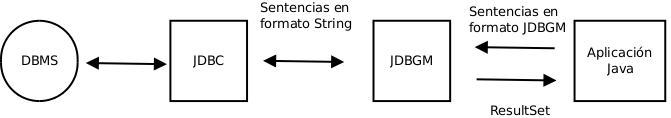
\includegraphics[width=0.85\textwidth]{figuras/jdbgm-overview.png}
  \caption{JDBGM dentro de una aplicación}
  \label{fig:jdbgm:overview}
\end{figure}

Así que \jj debe ser capaz de hacer dos tareas independientes pero relacionadas, en primer lugar debe proveer el almacenamiento de las sentencias de modo que puedan ser traducidas luego a el dialecto que corresponda y en segundo lugar proveer los métodos necesarios para comunicarse con el motor mediante \jd, podemos observar esquemáticamente la situación en la figura \figpage{fig:jdbgm:closerlook} que nos muestra la idea de independencia existente entre los dos módulos principales que se están exponiendo, el manejador de sentencias es totalmente independiente de la capa intermedia pues de lo que esta encargado es de proveer los métodos necesarios para ``armar las sentencias'' y traducirlas cuando sea requerido a el dialecto correspondiente, esta traducción lo que hace es convertir la sentencia almacenada a una cadena de texto la cual es entendible por \jd por lo que se podría obviar la capa intermedia que hace transparente su uso y usarlo directamente. En cambio la capa intermedia dependerá de el manejador de sentencias para poder proveer la independencia de dialectos que se quiere lograr y además este solo recibirá las sentencias compatibles con el formato propuesto por \jj por lo que a continuación se procederá a explicar la estructura propuesta para este manejador para que después se pueda explicar correctamente el funcionamiento de la capa intermedia.

\begin{figure}
  \centering
    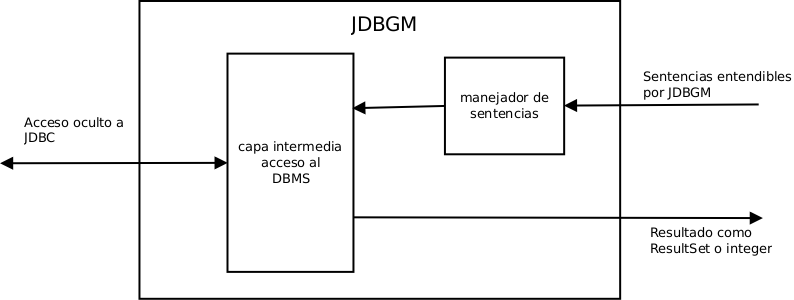
\includegraphics[width=0.85\textwidth]{figuras/jdbgm-closerlook.png}
  \caption{Vista abstracta del funcionamiento de JDBGM}
  \label{fig:jdbgm:closerlook}
\end{figure}

\section{Manejador de sentencias}
Como ya se dijo el manejador de sentencias debe ser capaz de almacenar las sentencias de forma desglosada así que pasemos a ver que se quiere lograr. Como una primer solución podemos pensar que una sentencia como la siguiente ``\verb=nombre_comando parametro opcion1 parametro1 opcion2 parametro2='' que se podría corresponder con la siguiente consulta ``\verb|SELECT * FROM table WHERE table.id=1|'', salvando ciertas reglas de construcción que en este momento no vienen al caso, puede ser almacenado en una clase que se corresponda con el siguiente esquema:

\begin{lstlisting}[title=Pseudocódigo de la estructura de dato que contiene la sentencia]
class Sentencia{
	nombre_comando;
	parametro;
	set_opcion1(parametro1);
	set_opcion2(parametro2);
	devolver_sentencia();
}
\end{lstlisting}
Como se ve es una idea bastante sencilla en la que la clase identificara la sentencia y sus opciones correspondientes serán nombres de atributos pues en definitiva lo que nos interesa de estas opciones son los valores que toman o si están presentes o no en la sentencia que se esta armando. Como clase de POO también debe ofrecer métodos para almacenar los valores que tomaran las opciones y es aquí donde empiezan a jugar las reglas dispuestas en el dialecto genérico que fue especificado en el capitulo \ref{capitulo:especificacion}, puesto que las opciones ofrecidas por cada sentencia no pueden ser libremente usadas es necesario que estos métodos restrinjan el modo en que se pueden usar ya sea limitando las posibilidades de el/los métodos o bien usando excepciones para detener la ejecución del programa, una explicación mas detallada del manejo de excepciones se vera en las secciones siguientes, cuando alguna acción ilegal sobre las sentencias ocurra.

Con esto ya se tiene una idea genérica de las clases que se quiere representen a las sentencias y teniendo en cuenta que cada una de estas clases representa a una sentencia diferente con un comportamiento diferente pero con similitudes es necesario recalcar que estas diferentes clases deben presentar las mismas similitudes, por ejemplo supóngase que los objetos \verb|select| y \verb|create| representan las sentencias SQL del mismo nombre las cuales precisan que se les asigne el nombre de la tabla sobre la que se esta trabajando entonces lo correcto sera que ambos objetos tengan un método de igual nombre y comportamiento igual como por ejemplo \verb=select.set_table_name("name_1")= y \verb=create.set_table_name("name_2")=. Es muy importante tener en cuenta esto puesto que facilitara el aprendizaje del uso de la API del manejador de sentencias que se esta proponiendo y además hará el uso de la misma mucho mas natural, con respecto a SQL. Antes de empezar a hablar de lleno de la arquitectura propuesta para el manejador de sentencia es necesario nombrar al paquete \cc de el cual se tomaron algunas ideas.

\subsection{El paquete \cc}
Este paquete que puede ser encontrado en \href{http://sourceforge.net}{SourceForge} en la siguiente dirección \url{http://sourceforge.net/projects/crossdb/} intenta solucionar el mismo problema que el manejador de sentencias aquí presentado tal como se puede observar en la pagina del proyecto que se resume en la siguiente oración:

\begin{center}
``To provide cross database tools for manipulating all major databases without having to worry about each vendors specific implementation.''
\end{center} 

Esta librería  usa la misma idea de ir generando bajo demanda las sentencias por lo que se la estudio y se llego a la conclusión de que podía servir como base para el manejador que se quiere implementar en este proyecto. Algunas consideraciones antes de avanzar:
\begin{itemize}
\item El paquete se distribuye bajo Apache Software License 1.1 por lo que no hay inconvenientes en reusar el código escrito, siempre y cuando se respeten las condiciones impuestas. Además esta licencia es compatible con GPL.
\item La ultima actualización del proyecto data el 23-08-2005 (la ultima modificación registrada en el repositorio svn) por lo que aparentemente el proyecto quedo en un punto muerto y en una versión beta básica según se puede ver al revisar el código.
\item Carece de una buena documentación pero el código es bastante entendible y mas aun después de venir estudiando una solución similar a la propuesta por \cc


\end{itemize}
Se puede resumir la estructura usada por esta librería en el gráfico \fullref{fig:crossdb:base-idea} que nos muestra que por cada sentencia existe una Interfaz \verb=Statement= que define el comportamiento de la misma, luego para esta interfaz base existe una implementación por defecto \verb=DefaultStatement= que implementa las funciones que son comunes a toda implementación que se pueda realizar de dicha interfaz, recordando que al trabajar con dialectos estamos trabajando con variaciones de un lenguaje base, y por cada una de estas implementaciones por defecto existe una implementación especifica \verb=SpecificStatement= que contempla las particularidades de un motor en particular sobre dicha sentencia. En la misma figura podemos observar como se conforma dicha arquitectura para la sentencia \verb=SELECT= con la clases \verb=SelectQuery= siendo la interfaz base, \verb=DefaultSelectQuery= siendo la implementación por defecto de dicha interfaz y \verb=OracleSelectQuery= una implementación especifica para el dialecto usado por Oracle.


%\begin{figure}
%  \centering
%    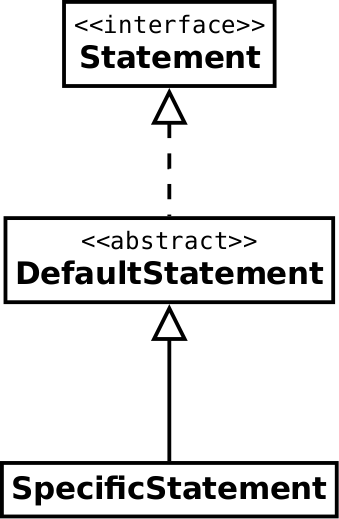
\includegraphics[width=0.2\textwidth]{figuras/crossdb-base-idea.png}
%  \caption{Vista abstracta de la arquitectura de crossdb}
%  \label{fig:crossdb:base-idea}
%\end{figure}
\begin{figure}
  \centering
  \subfloat[Idea base]{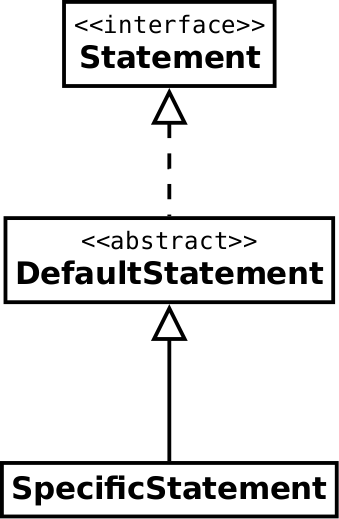
\includegraphics[width=0.2\textwidth]{figuras/crossdb-base-idea.png}} \label{fig:subfig:crossdb:base-idea}
  \qquad 
  \subfloat[Ejemplo con Select]{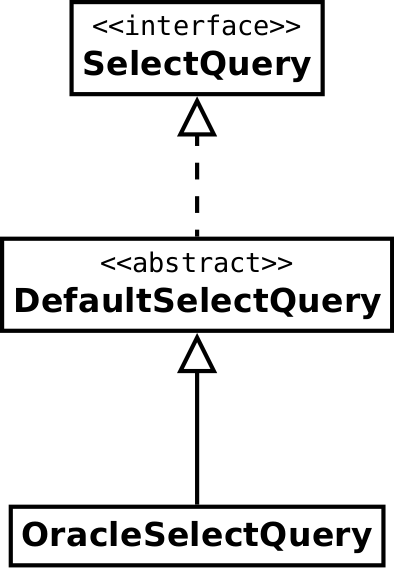
\includegraphics[width=0.2\textwidth]{figuras/crossdb-base-idea-select.png}} \label{fig:subfig:crossdb:base-idea-select}
  \caption{Vista abstracta de la arquitectura de crossdb}
  \label{fig:crossdb:base-idea}
\end{figure}

Además de las clases a las que se hizo referencia \cc usa otras auxiliares, como \verb=Column= que contiene los datos necesarios para especificar una columna o \verb=WhereClause= que representa una clausula \verb=WHERE=, necesarias para poder almacenar adecuadamente los datos para las sentencias que se están armando. También se implementaba la idea del patrón Factory pero de una manera muy básica. Terminado de presentar ligeramente este paquete sobre el cual se baso el diseño propuesto en este trabajo se pasara a exponer la arquitectura usada por el manejador de sentencias y su relación con las ideas tomadas de \cc.

\subsection{Diseño de el Manejador}


\section{JDBC y su envoltorio}
y otro
Java ya nos provee JDBC para acceder a las bases de datos, pero al hacer uso de el es necesario especificar con que motor se esta trabajando, para ejemplificar ello veamos el típico código que debemos escribir para conectarnos a una base de datos.

\begin{lstlisting}[title=Porción de codigo java para la conexión a una base de datos]
class conectDB(){
...

Class.forName("com.mysql.jdbc.Driver");
	Connection conexion = DriverManager.getConnection(
		"jdbc:mysql://localhost/AsistenciaAlumnos", "tester",
		"tester");
	Statement st = (Statement) conexion.createStatement();

...
}
\end{lstlisting}

En esta porción de código lo que se hace inicialmente es instanciar el driver, es decir crear el objeto driver, luego el método estático \verb=getConnection= de 	\verb=DriverManager= nos devuelve un objeto que representa la conexión al motor con el que se esta trabajando. Este objeto del tipo \verb=Connection= nos provee métodos para generar objetos \verb=Statement= que nos permite hacer consultas a la base de datos mediante las funciones que dispone. Una descripción mucho mas extensa de JDBC puede ser encontrada en la documentación disponible en la web de Oracle\citep{java:jdbc}.
Para nuestro proyecto necesitamos ocultar y simplificar el API de JDBC





\section{Abstracción de SQL}
